
%% bare_conf.tex
%% V1.3
%% 2007/01/11
%% by Michael Shell
%% See:
%% http://www.michaelshell.org/
%% for current contact information.
%%
%% This is a skeleton file demonstrating the use of IEEEtran.cls
%% (requires IEEEtran.cls version 1.7 or later) with an IEEE conference paper.
%%
%% Support sites:
%% http://www.michaelshell.org/tex/ieeetran/
%% http://www.ctan.org/tex-archive/macros/latex/contrib/IEEEtran/
%% and
%% http://www.ieee.org/

%%*************************************************************************
%% Legal Notice:
%% This code is offered as-is without any warranty either expressed or
%% implied; without even the implied warranty of MERCHANTABILITY or
%% FITNESS FOR A PARTICULAR PURPOSE!
%% User assumes all risk.
%% In no event shall IEEE or any contributor to this code be liable for
%% any damages or losses, including, but not limited to, incidental,
%% consequential, or any other damages, resulting from the use or misuse
%% of any information contained here.
%%
%% All comments are the opinions of their respective authors and are not
%% necessarily endorsed by the IEEE.
%%
%% This work is distributed under the LaTeX Project Public License (LPPL)
%% ( http://www.latex-project.org/ ) version 1.3, and may be freely used,
%% distributed and modified. A copy of the LPPL, version 1.3, is included
%% in the base LaTeX documentation of all distributions of LaTeX released
%% 2003/12/01 or later.
%% Retain all contribution notices and credits.
%% ** Modified files should be clearly indicated as such, including  **
%% ** renaming them and changing author support contact information. **
%%
%% File list of work: IEEEtran.cls, IEEEtran_HOWTO.pdf, bare_adv.tex,
%%                    bare_conf.tex, bare_jrnl.tex, bare_jrnl_compsoc.tex
%%*************************************************************************

% *** Authors should verify (and, if needed, correct) their LaTeX system  ***
% *** with the testflow diagnostic prior to trusting their LaTeX platform ***
% *** with production work. IEEE's font choices can trigger bugs that do  ***
% *** not appear when using other class files.                            ***
% The testflow support page is at:
% http://www.michaelshell.org/tex/testflow/



% Note that the a4paper option is mainly intended so that authors in
% countries using A4 can easily print to A4 and see how their papers will
% look in print - the typesetting of the document will not typically be
% affected with changes in paper size (but the bottom and side margins will).
% Use the testflow package mentioned above to verify correct handling of
% both paper sizes by the user's LaTeX system.
%
% Also note that the "draftcls" or "draftclsnofoot", not "draft", option
% should be used if it is desired that the figures are to be displayed in
% draft mode.
%
\documentclass[10pt,conference]{cls/IEEEtran}
% Add the compsoc option for Computer Society conferences.
%
% If IEEEtran.cls has not been installed into the LaTeX system files,
% manually specify the path to it like:
% \documentclass[conference]{../sty/IEEEtran}





% Some very useful LaTeX packages include:
% (uncomment the ones you want to load)


% *** MISC UTILITY PACKAGES ***
%
%\usepackage{ifpdf}
% Heiko Oberdiek's ifpdf.sty is very useful if you need conditional
% compilation based on whether the output is pdf or dvi.
% usage:
% \ifpdf
%   % pdf code
% \else
%   % dvi code
% \fi
% The latest version of ifpdf.sty can be obtained from:
% http://www.ctan.org/tex-archive/macros/latex/contrib/oberdiek/
% Also, note that IEEEtran.cls V1.7 and later provides a builtin
% \ifCLASSINFOpdf conditional that works the same way.
% When switching from latex to pdflatex and vice-versa, the compiler may
% have to be run twice to clear warning/error messages.






% *** CITATION PACKAGES ***
%
\usepackage{cite}
% cite.sty was written by Donald Arseneau
% V1.6 and later of IEEEtran pre-defines the format of the cite.sty package
% \cite{} output to follow that of IEEE. Loading the cite package will
% result in citation numbers being automatically sorted and properly
% "compressed/ranged". e.g., [1], [9], [2], [7], [5], [6] without using
% cite.sty will become [1], [2], [5]--[7], [9] using cite.sty. cite.sty's
% \cite will automatically add leading space, if needed. Use cite.sty's
% noadjust option (cite.sty V3.8 and later) if you want to turn this off.
% cite.sty is already installed on most LaTeX systems. Be sure and use
% version 4.0 (2003-05-27) and later if using hyperref.sty. cite.sty does
% not currently provide for hyperlinked citations.
% The latest version can be obtained at:
% http://www.ctan.org/tex-archive/macros/latex/contrib/cite/
% The documentation is contained in the cite.sty file itself.






\usepackage{graphicx}
% *** GRAPHICS RELATED PACKAGES ***
%
%\ifCLASSINFOpdf
  % \usepackage[pdftex]{graphicx}
  % declare the path(s) where your graphic files are
  % \graphicspath{{../pdf/}{../jpeg/}}
  % and their extensions so you won't have to specify these with
  % every instance of \includegraphics
  % \DeclareGraphicsExtensions{.pdf,.jpeg,.png}
%\else
  % or other class option (dvipsone, dvipdf, if not using dvips). graphicx
  % will default to the driver specified in the system graphics.cfg if no
  % driver is specified.
  % \usepackage[dvips]{graphicx}
  % declare the path(s) where your graphic files are
  % \graphicspath{{../eps/}}
  % and their extensions so you won't have to specify these with
  % every instance of \includegraphics
  % \DeclareGraphicsExtensions{.eps}
%\fi
% graphicx was written by David Carlisle and Sebastian Rahtz. It is
% required if you want graphics, photos, etc. graphicx.sty is already
% installed on most LaTeX systems. The latest version and documentation can
% be obtained at:
% http://www.ctan.org/tex-archive/macros/latex/required/graphics/
% Another good source of documentation is "Using Imported Graphics in
% LaTeX2e" by Keith Reckdahl which can be found as epslatex.ps or
% epslatex.pdf at: http://www.ctan.org/tex-archive/info/
%
% latex, and pdflatex in dvi mode, support graphics in encapsulated
% postscript (.eps) format. pdflatex in pdf mode supports graphics
% in .pdf, .jpeg, .png and .mps (metapost) formats. Users should ensure
% that all non-photo figures use a vector format (.eps, .pdf, .mps) and
% not a bitmapped formats (.jpeg, .png). IEEE frowns on bitmapped formats
% which can result in "jaggedy"/blurry rendering of lines and letters as
% well as large increases in file sizes.
%
% You can find documentation about the pdfTeX application at:
% http://www.tug.org/applications/pdftex





% *** MATH PACKAGES ***
%
\usepackage[cmex10]{amsmath}
% A popular package from the American Mathematical Society that provides
% many useful and powerful commands for dealing with mathematics. If using
% it, be sure to load this package with the cmex10 option to ensure that
% only type 1 fonts will utilized at all point sizes. Without this option,
% it is possible that some math symbols, particularly those within
% footnotes, will be rendered in bitmap form which will result in a
% document that can not be IEEE Xplore compliant!
%
% Also, note that the amsmath package sets \interdisplaylinepenalty to 10000
% thus preventing page breaks from occurring within multiline equations. Use:
%\interdisplaylinepenalty=2500
% after loading amsmath to restore such page breaks as IEEEtran.cls normally
% does. amsmath.sty is already installed on most LaTeX systems. The latest
% version and documentation can be obtained at:
% http://www.ctan.org/tex-archive/macros/latex/required/amslatex/math/





% *** SPECIALIZED LIST PACKAGES ***
%
\usepackage{algorithm}
\usepackage{algorithmicx}
\usepackage{algpseudocode}
%\algrenewcommand\algorithmicrequire{\textbf{Input}}
%\algrenewcommand\algorithmicensure{\textbf{Output}}
% algorithmic.sty was written by Peter Williams and Rogerio Brito.
% This package provides an algorithmic environment fo describing algorithms.
% You can use the algorithmic environment in-text or within a figure
% environment to provide for a floating algorithm. Do NOT use the algorithm
% floating environment provided by algorithm.sty (by the same authors) or
% algorithm2e.sty (by Christophe Fiorio) as IEEE does not use dedicated
% algorithm float types and packages that provide these will not provide
% correct IEEE style captions. The latest version and documentation of
% algorithmic.sty can be obtained at:
% http://www.ctan.org/tex-archive/macros/latex/contrib/algorithms/
% There is also a support site at:
% http://algorithms.berlios.de/index.html
% Also of interest may be the (relatively newer and more customizable)
% algorithmicx.sty package by Szasz Janos:
% http://www.ctan.org/tex-archive/macros/latex/contrib/algorithmicx/




% *** ALIGNMENT PACKAGES ***
%
%\usepackage{array}
% Frank Mittelbach's and David Carlisle's array.sty patches and improves
% the standard LaTeX2e array and tabular environments to provide better
% appearance and additional user controls. As the default LaTeX2e table
% generation code is lacking to the point of almost being broken with
% respect to the quality of the end results, all users are strongly
% advised to use an enhanced (at the very least that provided by array.sty)
% set of table tools. array.sty is already installed on most systems. The
% latest version and documentation can be obtained at:
% http://www.ctan.org/tex-archive/macros/latex/required/tools/


%\usepackage{mdwmath}
%\usepackage{mdwtab}
% Also highly recommended is Mark Wooding's extremely powerful MDW tools,
% especially mdwmath.sty and mdwtab.sty which are used to format equations
% and tables, respectively. The MDWtools set is already installed on most
% LaTeX systems. The lastest version and documentation is available at:
% http://www.ctan.org/tex-archive/macros/latex/contrib/mdwtools/


% IEEEtran contains the IEEEeqnarray family of commands that can be used to
% generate multiline equations as well as matrices, tables, etc., of high
% quality.


%\usepackage{eqparbox}
% Also of notable interest is Scott Pakin's eqparbox package for creating
% (automatically sized) equal width boxes - aka "natural width parboxes".
% Available at:
% http://www.ctan.org/tex-archive/macros/latex/contrib/eqparbox/





% *** SUBFIGURE PACKAGES ***
%\usepackage[tight,footnotesize]{subfigure}
% subfigure.sty was written by Steven Douglas Cochran. This package makes it
% easy to put subfigures in your figures. e.g., "Figure 1a and 1b". For IEEE
% work, it is a good idea to load it with the tight package option to reduce
% the amount of white space around the subfigures. subfigure.sty is already
% installed on most LaTeX systems. The latest version and documentation can
% be obtained at:
% http://www.ctan.org/tex-archive/obsolete/macros/latex/contrib/subfigure/
% subfigure.sty has been superceeded by subfig.sty.



%\usepackage[caption=false]{caption}
\usepackage{subfig}
% subfig.sty, also written by Steven Douglas Cochran, is the modern
% replacement for subfigure.sty. However, subfig.sty requires and
% automatically loads Axel Sommerfeldt's caption.sty which will override
% IEEEtran.cls handling of captions and this will result in nonIEEE style
% figure/table captions. To prevent this problem, be sure and preload
% caption.sty with its "caption=false" package option. This is will preserve
% IEEEtran.cls handing of captions. Version 1.3 (2005/06/28) and later
% (recommended due to many improvements over 1.2) of subfig.sty supports
% the caption=false option directly:
%\usepackage[caption=false,font=footnotesize]{subfig}
%
% The latest version and documentation can be obtained at:
% http://www.ctan.org/tex-archive/macros/latex/contrib/subfig/
% The latest version and documentation of caption.sty can be obtained at:
% http://www.ctan.org/tex-archive/macros/latex/contrib/caption/




% *** FLOAT PACKAGES ***
%
%\usepackage{fixltx2e}
% fixltx2e, the successor to the earlier fix2col.sty, was written by
% Frank Mittelbach and David Carlisle. This package corrects a few problems
% in the LaTeX2e kernel, the most notable of which is that in current
% LaTeX2e releases, the ordering of single and double column floats is not
% guaranteed to be preserved. Thus, an unpatched LaTeX2e can allow a
% single column figure to be placed prior to an earlier double column
% figure. The latest version and documentation can be found at:
% http://www.ctan.org/tex-archive/macros/latex/base/



%\usepackage{stfloats}
% stfloats.sty was written by Sigitas Tolusis. This package gives LaTeX2e
% the ability to do double column floats at the bottom of the page as well
% as the top. (e.g., "\begin{figure*}[!b]" is not normally possible in
% LaTeX2e). It also provides a command:
%\fnbelowfloat
% to enable the placement of footnotes below bottom floats (the standard
% LaTeX2e kernel puts them above bottom floats). This is an invasive package
% which rewrites many portions of the LaTeX2e float routines. It may not work
% with other packages that modify the LaTeX2e float routines. The latest
% version and documentation can be obtained at:
% http://www.ctan.org/tex-archive/macros/latex/contrib/sttools/
% Documentation is contained in the stfloats.sty comments as well as in the
% presfull.pdf file. Do not use the stfloats baselinefloat ability as IEEE
% does not allow \baselineskip to stretch. Authors submitting work to the
% IEEE should note that IEEE rarely uses double column equations and
% that authors should try to avoid such use. Do not be tempted to use the
% cuted.sty or midfloat.sty packages (also by Sigitas Tolusis) as IEEE does
% not format its papers in such ways.





% *** PDF, URL AND HYPERLINK PACKAGES ***
%
\usepackage{url}
\usepackage{booktabs}
% url.sty was written by Donald Arseneau. It provides better support for
% handling and breaking URLs. url.sty is already installed on most LaTeX
% systems. The latest version can be obtained at:
% http://www.ctan.org/tex-archive/macros/latex/contrib/misc/
% Read the url.sty source comments for usage information. Basically,
% \url{my_url_here}.





% *** Do not adjust lengths that control margins, column widths, etc. ***
% *** Do not use packages that alter fonts (such as pslatex).         ***
% There should be no need to do such things with IEEEtran.cls V1.6 and later.
% (Unless specifically asked to do so by the journal or conference you plan
% to submit to, of course. )


% correct bad hyphenation here
\hyphenation{op-tical net-works semi-conduc-tor}


\begin{document}
%
% paper title
% can use linebreaks \\ within to get better formatting as desired
\title{Uno: A Privacy-Aware Distributed Storage and \\Replication Middleware for Heterogeneous Computing Platforms}

% author names and affiliations
% use a multiple column layout for up to three different
% affiliations
\author{
\IEEEauthorblockN{Jilong Liao}
\IEEEauthorblockA{Department of Electrical Engineering \\and Computer Science\\
University of Tennessee,\\ Knoxville TN, 37996\\
Email: jliao2@utk.edu}
\and
\IEEEauthorblockN{Kefa Lu}
\IEEEauthorblockA{Department of Electrical Engineering \\and Computer Science\\
University of Tennessee,\\ Knoxville TN, 37996\\
Email: klu3@utk.edu}
\and
\IEEEauthorblockN{Qing Cao}
\IEEEauthorblockA{Department of Electrical Engineering \\and Computer Science\\
University of Tennessee,\\ Knoxville TN, 37996\\
Email: cao@utk.edu}
}

% conference papers do not typically use \thanks and this command
% is locked out in conference mode. If really needed, such as for
% the acknowledgment of grants, issue a \IEEEoverridecommandlockouts
% after \documentclass

% for over three affiliations, or if they all won't fit within the width
% of the page, use this alternative format:
%
%\author{\IEEEauthorblockN{Michael Shell\IEEEauthorrefmark{1},
%Homer Simpson\IEEEauthorrefmark{2},
%James Kirk\IEEEauthorrefmark{3},
%Montgomery Scott\IEEEauthorrefmark{3} and
%Eldon Tyrell\IEEEauthorrefmark{4}}
%\IEEEauthorblockA{\IEEEauthorrefmark{1}School of Electrical and Computer Engineering\\
%Georgia Institute of Technology,
%Atlanta, Georgia 30332--0250\\ Email: see http://www.michaelshell.org/contact.html}
%\IEEEauthorblockA{\IEEEauthorrefmark{2}Twentieth Century Fox, Springfield, USA\\
%Email: homer@thesimpsons.com}
%\IEEEauthorblockA{\IEEEauthorrefmark{3}Starfleet Academy, San Francisco, California 96678-2391\\
%Telephone: (800) 555--1212, Fax: (888) 555--1212}
%\IEEEauthorblockA{\IEEEauthorrefmark{4}Tyrell Inc., 123 Replicant Street, Los Angeles, California 90210--4321}}




% use for special paper notices
%\IEEEspecialpapernotice{(Invited Paper)}




% make the title area
\maketitle


\begin{abstract}
Cloud computing is an emerging research area that has drawn considerable interest in recent years. However, the current infrastructure raises significant concerns about how to protect users' privacy, in part due to that users are storing their data in the cloud vendors' servers. In this paper, we address this challenge by proposing and implementing a novel middleware, called \emph{Uno}, which separates the storage of physical data and their associated metadata. In our design, users' physical data are stored locally on those devices under a user's full control, while their metadata can be uploaded to the commercial cloud. To ensure the reliability of users' data, we develop a novel fine-grained file replication algorithm that exploits both data access patterns and device state patterns. Based on a quantitative analysis of the data set from Rice University~\cite{shepard2011livelab}, this algorithm replicates data intelligently in different time slots, so that it can not only significantly improve data availability, but also achieve a satisfactory performance on load balancing and storage diversification. We implement the Uno system on a heterogeneous testbed composed of both host servers and mobile devices, and demonstrate the programmability of Uno through implementation and evaluation of two sample applications, \emph{Uno@Home} and \emph{Uno@Sense}.
\end{abstract}

% IEEEtran.cls defaults to using nonbold math in the Abstract.
% This preserves the distinction between vectors and scalars. However,
% if the conference you are submitting to favors bold math in the abstract,
% then you can use LaTeX's standard command \boldmath at the very start
% of the abstract to achieve this. Many IEEE journals/conferences frown on
% math in the abstract anyway.

% no keywords


% For peer review papers, you can put extra information on the cover
% page as needed:
% \ifCLASSOPTIONpeerreview
% \begin{center} \bfseries EDICS Category: 3-BBND \end{center}
% \fi
%
% For peerreview papers, this IEEEtran command inserts a page break and
% creates the second title. It will be ignored for other modes.
\IEEEpeerreviewmaketitle

\section{Introduction}\label{sec:introduction}
Cloud computing has become one of the most powerful tools which could potentially help people solve some extremely hard problems. The computation and storage resource in the cloud are relatively cheap and convenient comparing to build something from the scratch. Besides, the public cloud vendors, like Amazon and Google, have made its own powerful computation and storage infrastructure available to the public via cloud computing service. Those cloud vendors provide either virtual machines or pre-defined cloud APIs to help people build application on top of their cloud very easy and fast.

By the booming time of cloud computing, people may have the chance to rethink of the way to solve some existing hard problems in computer science. The hard problems (usually belongs to the NP-Complete category like 3-SAT) often require exponential computation time to traverse the solution space in a brute-force manner. In addition, people may need to solve the same types of problems again and again in different instance. Some instances or subproblems possibly have been solved by others. Therefore, we come to the idea that \emph{cache the existing solutions to those problems and query the solutions before we solve any other problems}. 

One immediate challenge of this idea is the storage requirement. Even the same type of problem, e.g. 3-SAT, could have numerous problem instance, which may require several disks to store them, let alone we have many different types of hard problems. Cloud computing, at this point, could be a proper plagiarism because it is much less expensive to build a large scale storage and its management system. The other challenge is how we abstract the hard problems in a way that the platform we build could be more general to many different type of hard problems.

In this document, we propose \emph{CloudCache} framework which is built on top of general cloud computing platform and provides the interface to query, cache and solve hard problems in an easier way. The CloudCache framework abstracts the \emph{problem-solution} pair into \emph{key-value} objects, and uses some object storage system to cache existing problems and solutions. Further, the CloudCache framework provides a general problem solving interface \emph{kernel-solver}, so that the developer can easily write a problem's solution and solve it within the CloudCache's framework. CloudCache executes kernel-solver in a distributed way which tries to maximize the framework's problem solving throughput.

The rest of the document is arranged in the following way: Section~\ref{sec:design} describes the design and reasoning of the CloudCache framework; Section~\ref{sec:implementation} shows the implementations of the framework; Section~\ref{sec:evaluation} deploys the framework in Amazon EC2 and solves $1,000,000$ 3-SAT problem instances; Finally, we discuss some potential improvements and conclusion in Section~\ref{sec:conclusion}.

\input{tex/relatedwork}
\section{Framework Design}\label{sec:design}
\subsection{The Problem-Solution Abstraction}
Many different types of hard problem we encounter have various input structure. For instance, 3-SAT problem input a logic expression while Clique problem needs a graph structure. Those different types of inputs brings the challenges to the CloudCache framework, because it is possible the CloudCache framework host many different types of problems and solutions and the cache query operation need to find the exact solutions for a certain problem. If we do not have a uniform structure for the all problems, the complexity in localizing problems and its solutions will be very large.

In CloudCache framework, we propose the general \emph{key-value} objects as the abstractions of problem-solutions where problems are the \emph{key} objects and solutions are the \emph{value} objects. To store the key-value objects in the general storage system (e.g. MySQL, Redis and MongoDB), we serialize the keys and values to strings. In this way, the general storage system can easily index, search and maintain the problems and its solutions regardless what type of problem it is.

For a specific problem, like the 3-SAT problem, the developers can define their data structure at their own convenience. The CloudCache framework's cache \emph{query()} and \emph{push()} APIs will first serialize the developer defined data structure when calling both APIs.

\subsection{Core System Design}
\begin{figure}
\centering
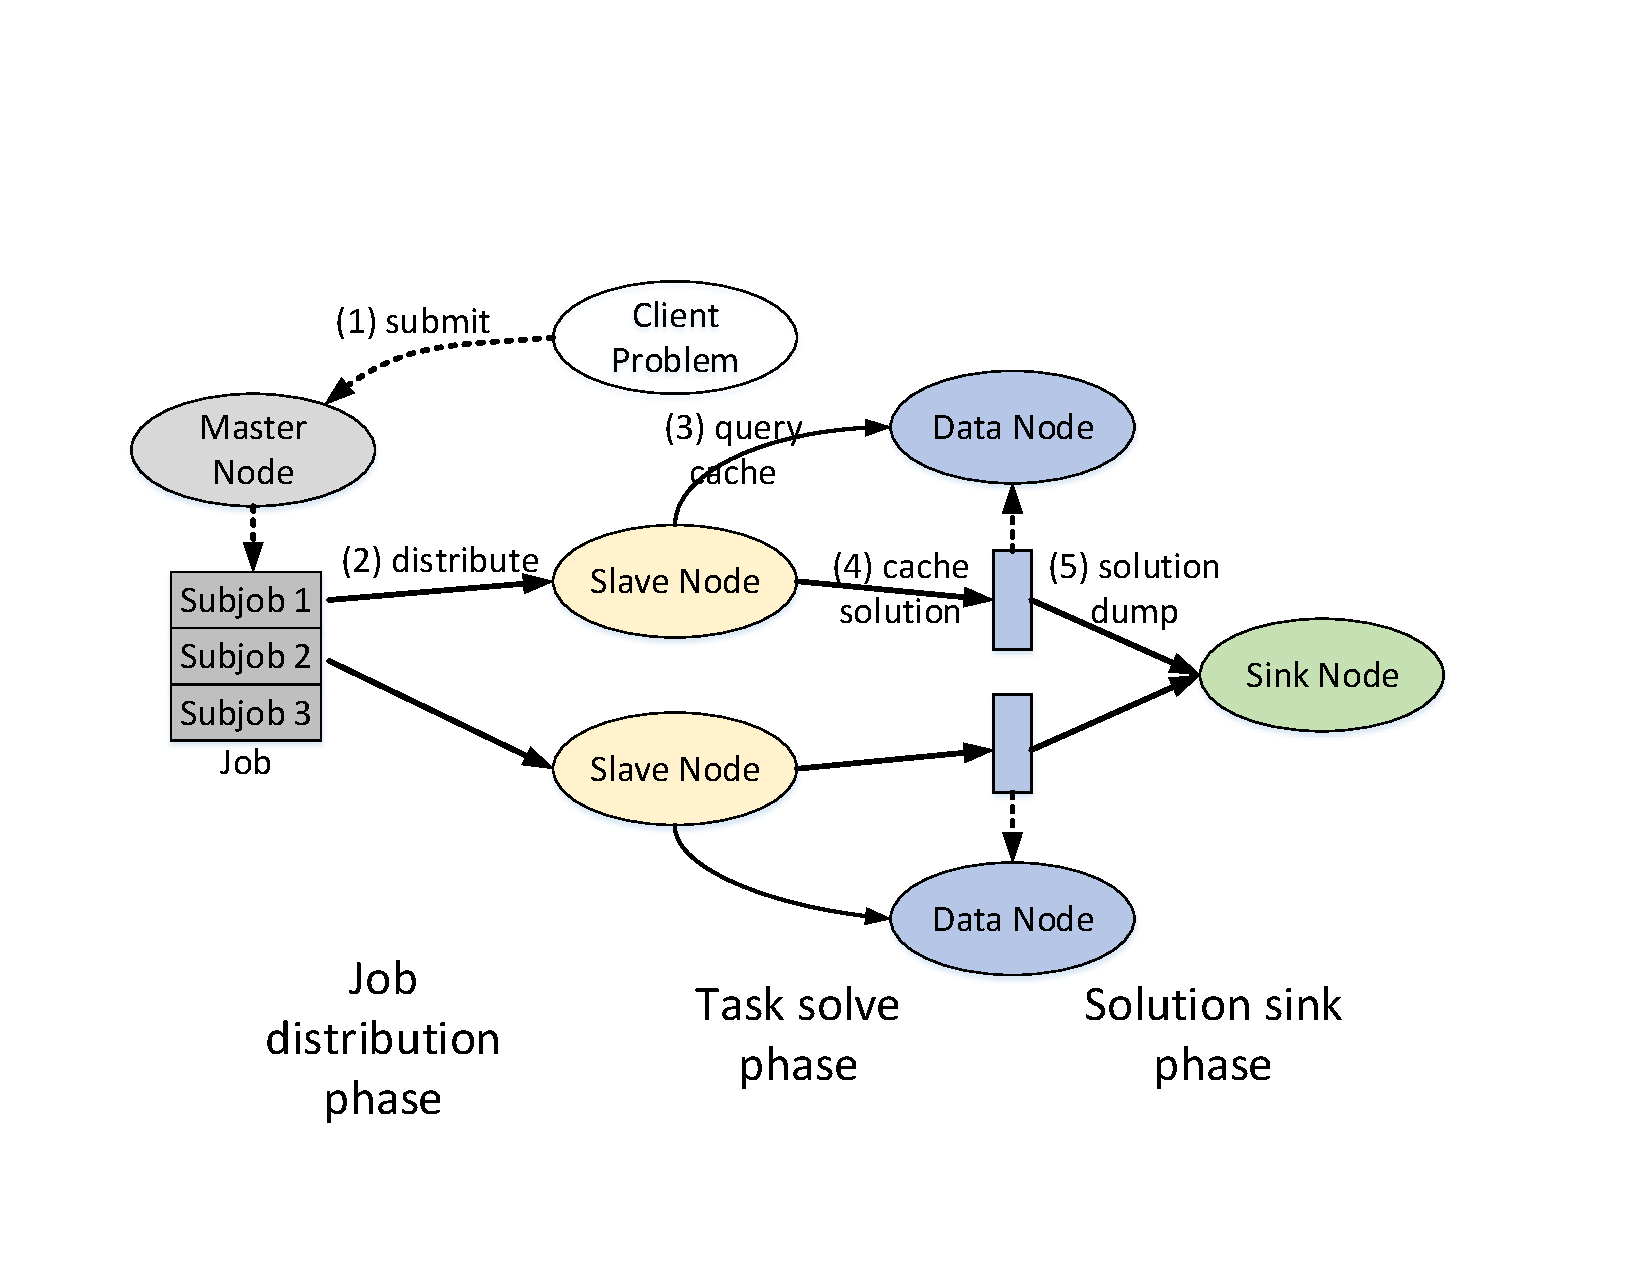
\includegraphics[width=0.5\textwidth]{pics/workflow.pdf}
\caption{The Logic Diagram of CloudCache}
\label{fig:logic}
\end{figure}

The CloudCache framework (Fig.~\ref{fig:logic}) includes four types of nodes and three computation phases in the cloud infrastructure. The nodes are \emph{Master Node}, \emph{Slave Node}, \emph{Data Node} and \emph{Sink Node}; the three phases are \emph{Job Distribution Phase}, \emph{Task Solve Phase} and \emph{Solution Sink Phase}. In addition, the \emph{Client Problem} exists outside of the cloud infrastructure which needs to be submitted into the CloudCache framework.

The Master Node is the central control component of the whole framework. It accepts the job submission from the client problem and split the the job into several subjobs. Those subjobs will later be distributed to different Slave Nodes. For each of the task in the subjob which the Slave Node is received from the Master Node, the Slave Node will initiate a \emph{kernel-solver} for the task. The kernel-solver is the single execution box defined by the developers for a problem which performs the cache query and solve functions. When the kernel-solver starts execution, it uses the \emph{query()} API to check if the current problem already has a solution in the CloudCache. The query API uses a \emph{hash} function to select the dedicated Data Node where a part of existing solutions are stored. Once the Data Node has been identified, the Data Node will response with a solution if the problem has been solved or a NULL value.

Whether the kernel-solver find the existing solutions or solve it by itself, the solution for the assigned problem will be cached in the Data Node, selected by the same hash function. We use a hash function to shard the queries because we consider the load balance of the Data Node which is much busier than Slave Node or Master Node in the system. In addition to cache the problem's solution, the solution needs to report to the Sink Node where the client program will come and retrieve the final results for all tasks in the job after the system finish the job. Note that we only have single Sink Node while the each kernel-solver will report its results to the Sink Node, the load at the Sink Node is significant which defects the whole system's throughput. Therefore, we have a small optimization that buffers the solution in each Slave Node until certain amount, then the Slave Node will report the buffered results together at once.

\subsection{Framework Generalness}
An expected design goal of CloudCache is the generalness, we want to make this framework to be a proper and simple approach to solve many different types of hard problems in the cloud. According to the design, only two things need to be defined by the developer before using the framework. First, the problem and solution's data structure; second, the kernel-solver of the problem, namely when to query the cache and when to solve the problem by itself. After finishing the two parts, the developer can submit a batch of problem as a job to the Master Node, where each problem is regarded as a task. Then the framework will start executing the batch job. In this section, we will show two hard problems' solution using CloudCache framework.

\subsubsection{3-SAT Problem}
The 3-SAT problem has an input of an boolean expression which contains many boolean variables' combinations in 3-conjunctive-normal-form clauses. For example, Eq.~\ref{eq:3-sat} shows an example 3-SAT problem which has $5$ boolean variables and has three clauses. For this problem, we use the expression vector as the key, but the vector is in a specific format. The boolean variable's index represents the variable itself in the vector, and the the index is set to be negative is the boolean variable has a ``not'' operator. The elements in expression are separated by a comma. Therefore, the \emph{key} for Eq.~\ref{eq:3-sat} is $[1,2,-3,2,3,4,3,-4,5]$.

\begin{equation}
Y = (x_1 \vee x_2 \vee \overline{x_3}) \wedge (x_2 \vee x_3 \vee x_4) \wedge (x_3 \vee \overline{x_4} \vee x_5)
\label{eq:3-sat}
\end{equation}

On the other hand, the solution of the problem is a vector of assignment, indicating each boolean variable's value as true or false. So for the 3-SAT problem instance in Eq.~\ref{eq:3-sat}, the \emph{value} is $[true, true, false, true, false]$. Once the key-value pair has been designed, we can move on to the \emph{kernel-solver} part.

The kernel-solver has two stages, the first stage is to check if the expression or any subexpression has been solved. We use a linear scan to do it by moving the head clause and check the subexpression between the head clause and the end one. For the example in Eq.~\ref{eq:3-sat}, we will check Eq.~\ref{eq:3-sat1},~\ref{eq:3-sat2},~\ref{eq:3-sat3}. If any of the subexpression has been solved, we will retrieve its solution then validate if the assignment can satisfy the whole expression. If so, we do not need a brute-force method to solve it again but just return the assignment in the cache. Otherwise, the brute-force method has to be run and we need to store the solved assignment in the cache. The two simple APIs to query and store key/value in the CloudCache make the operations very easy to do.

Note that we do not enumerate the possible combination of clauses in the expression to query the cache. The major reason is that most of the 3-SAT is not as hard as we may expect, thus the enumeration process may cost more time than a simple brute-force try. Besides, we cannot estimate the cache hit ratio for a clause combination ahead which may make the solution even slower as well.

\begin{equation}
Y = (x_1 \vee x_2 \vee \overline{x_3}) \wedge (x_2 \vee x_3 \vee x_4) \wedge (x_3 \vee \overline{x_4} \vee x_5)
\label{eq:3-sat1}
\end{equation}
\begin{equation}
Y = (x_2 \vee x_3 \vee x_4) \wedge (x_3 \vee \overline{x_4} \vee x_5)
\label{eq:3-sat2}
\end{equation}
\begin{equation}
Y = (x_3 \vee \overline{x_4} \vee x_5)
\label{eq:3-sat3}
\end{equation}


\subsubsection{k-coloring Problem}
The graph's k-coloring problem is to find a color assignment strategy that mark the vertex of the graph so that no adjacent vertex share the same color by using no more than k different colors. The problem is also a classic NP-Complete problem, the exact solution is a brute-force one by enumerating the $k^n$ assignments and validate them.

Similarly, we first need to abstract the problem-solution pairs. For the problem, we use a matrix $\mathbf{R}_{n\times n}$ to represent the graph which is the \emph{key}, and the \emph{value} is the color assignment vector $\mathbf{a} = [a_1, a_2, ..., a_n]$ where $n$ is the number of vertex in the graph.

The kernel-solver is also using a linear scan to all the vertices. For each vertex, we remove the edges connected to the vertex, then we have a new adjacent matrix $\hat{\mathbf{R}}_{(n-1)\times (n-1)}$ which is actually a subgraph of the original one. For this subgraph, we query the CloudCache to retrieve the existing color assignment. If success, we need to validate the assignment by enumerating the color of the removed vertex combining with the existing solution to see if the complete assignment can fit into the original graph. If so, we can cache the solution; if not, we continue removing another vertex in $\mathbf{R}_{n\times n}$ until we scan all the vertices one time. If cache is not working at all, the brute-force solver is triggered. 

\input{tex/infra}
\section{Evaluations} \label{sec:evaluation}

\input{tex/case-study}
\section{Conclusion}\label{sec:conclusion}
In this document, we describe the design and implementation of CloudCache framework. Through the evaluation, we find that the advantages of CloudCache framework has larger margin for the hard solving problem instances. We also look into the generalness of the framework by designing the solutions for the \emph{k-coloring} problem in the graph. The the solution paradigm fits into the problem very well, which reinforce the advantages of CloudCache framework. Finally, the system performance in CPU and network-in/out evaluation provides us a good fingerprints of the CloudCache framework as a whole.



% An example of a floating figure using the graphicx package.
% Note that \label must occur AFTER (or within) \caption.
% For figures, \caption should occur after the \includegraphics.
% Note that IEEEtran v1.7 and later has special internal code that
% is designed to preserve the operation of \label within \caption
% even when the captionsoff option is in effect. However, because
% of issues like this, it may be the safest practice to put all your
% \label just after \caption rather than within \caption{}.
%
% Reminder: the "draftcls" or "draftclsnofoot", not "draft", class
% option should be used if it is desired that the figures are to be
% displayed while in draft mode.
%
%\begin{figure}[!t]
%\centering
%\includegraphics[width=2.5in]{myfigure}
% where an .eps filename suffix will be assumed under latex,
% and a .pdf suffix will be assumed for pdflatex; or what has been declared
% via \DeclareGraphicsExtensions.
%\caption{Simulation Results}
%\label{fig_sim}
%\end{figure}

% Note that IEEE typically puts floats only at the top, even when this
% results in a large percentage of a column being occupied by floats.


% An example of a double column floating figure using two subfigures.
% (The subfig.sty package must be loaded for this to work.)
% The subfigure \label commands are set within each subfloat command, the
% \label for the overall figure must come after \caption.
% \hfil must be used as a separator to get equal spacing.
% The subfigure.sty package works much the same way, except \subfigure is
% used instead of \subfloat.
%
%\begin{figure*}[!t]
%\centerline{\subfloat[Case I]\includegraphics[width=2.5in]{subfigcase1}%
%\label{fig_first_case}}
%\hfil
%\subfloat[Case II]{\includegraphics[width=2.5in]{subfigcase2}%
%\label{fig_second_case}}}
%\caption{Simulation results}
%\label{fig_sim}
%\end{figure*}
%
% Note that often IEEE papers with subfigures do not employ subfigure
% captions (using the optional argument to \subfloat), but instead will
% reference/describe all of them (a), (b), etc., within the main caption.


% An example of a floating table. Note that, for IEEE style tables, the
% \caption command should come BEFORE the table. Table text will default to
% \footnotesize as IEEE normally uses this smaller font for tables.
% The \label must come after \caption as always.
%
%\begin{table}[!t]
%% increase table row spacing, adjust to taste
%\renewcommand{\arraystretch}{1.3}
% if using array.sty, it might be a good idea to tweak the value of
% \extrarowheight as needed to properly center the text within the cells
%\caption{An Example of a Table}
%\label{table_example}
%\centering
%% Some packages, such as MDW tools, offer better commands for making tables
%% than the plain LaTeX2e tabular which is used here.
%\begin{tabular}{|c||c|}
%\hline
%One & Two\\
%\hline
%Three & Four\\
%\hline
%\end{tabular}
%\end{table}


% Note that IEEE does not put floats in the very first column - or typically
% anywhere on the first page for that matter. Also, in-text middle ("here")
% positioning is not used. Most IEEE journals/conferences use top floats
% exclusively. Note that, LaTeX2e, unlike IEEE journals/conferences, places
% footnotes above bottom floats. This can be corrected via the \fnbelowfloat
% command of the stfloats package.







% conference papers do not normally have an appendix


% use section* for acknowledgement







% trigger a \newpage just before the given reference
% number - used to balance the columns on the last page
% adjust value as needed - may need to be readjusted if
% the document is modified later
%\IEEEtriggeratref{8}
% The "triggered" command can be changed if desired:
%\IEEEtriggercmd{\enlargethispage{-5in}}

% references section

% can use a bibliography generated by BibTeX as a .bbl file
% BibTeX documentation can be easily obtained at:
% http://www.ctan.org/tex-archive/biblio/bibtex/contrib/doc/
% The IEEEtran BibTeX style support page is at:
% http://www.michaelshell.org/tex/ieeetran/bibtex/
%\bibliographystyle{IEEEtran}
% argument is your BibTeX string definitions and bibliography database(s)
%\bibliography{IEEEabrv,ref.bib}
%
% <OR> manually copy in the resultant .bbl file
% set second argument of \begin to the number of references
% (used to reserve space for the reference number labels box)
%\begin{thebibliography}{1}
%\bibliography{}
%\end{thebibliography}

{\footnotesize
\bibliographystyle{IEEEtran}
\bibliography{reference}}  % sigproc.bib is the name of the Bibliography in this case

%\bibliographystyle{IEEEtran}
%\bibliography{ref}


% that's all folks
\end{document}


